\documentclass[10pt]{article}

% Lines beginning with the percent sign are comments
% This file has been commented to help you understand more about LaTeX

% DO NOT EDIT THE LINES BETWEEN THE TWO LONG HORIZONTAL LINES

%---------------------------------------------------------------------------------------------------------

% Packages add extra functionality.
\usepackage{
	times,
	graphicx,
	epstopdf,
	fancyhdr,
	amsfonts,
	amsthm,
	amsmath,
	algorithm,
	algorithmic,
	xspace,
	hyperref}
\usepackage[left=1in,top=1in,right=1in,bottom=1in]{geometry}
\usepackage{sect sty}	%For centering section headings
\usepackage{enumerate}	%Allows more labeling options for enumerate environments 
\usepackage{epsfig}
\usepackage[space]{grffile}
\usepackage{booktabs}
\usepackage{amsmath}
\usepackage[super]{nth}
\usepackage{array}

% This will set LaTeX to look for figures in the same directory as the .tex file
\graphicspath{.} % The dot means current directory.

\pagestyle{fancy}

\lhead{\YOURID}
\chead{\MyLang: Language Specification}
\rhead{\today}
\lfoot{CSCI 334: Principles of Programming Languages}
\cfoot{\thepage}
\rfoot{Spring 2022}

% Some commands for changing header and footer format
\renewcommand{\headrulewidth}{0.4pt}
\renewcommand{\headwidth}{\textwidth}
\renewcommand{\footrulewidth}{0.4pt}

% These let you use common environments
\newtheorem{claim}{Claim}
\newtheorem{definition}{Definition}
\newtheorem{theorem}{Theorem}
\newtheorem{lemma}{Lemma}
\newtheorem{observation}{Observation}
\newtheorem{question}{Question}

\setlength{\parindent}{0cm}
%---------------------------------------------------------------------------------------------------------

% DON'T CHANGE ANYTHING ABOVE HERE

% Edit below as instructed
\usepackage{adjustbox}
\newcommand{\MyLang}{PixelPunk}	% Replace MyLang with your language name #
\newcommand{\PartnerOne}{Max Kan}	% Replace PartnerOne with your name #
\newcommand{\PartnerTwo}{Rijul Jain}	% Replace PartnerTwo with your partner's name #
\newcommand{\YOURID}{\PartnerOne{} + \PartnerTwo{}} % Remove \PartnerTwo if working alone.


\title{\MyLang: Language Specification}
\date{Spring 2022}
\author{\PartnerOne{} and \PartnerTwo{}} % Remove \PartnerTwo if working alone.

\begin{document}
\maketitle

\vspace{\baselineskip}	% Add some vertical space

% Refer to the lab handouts to determine what should go in each of these sections.  Each lab is additive.  So lab 8 should include everything you wrote in lab 7.  Lab 9 should include everything you wrote in lab 8, etc.

\section{Introduction}
    Collins Dictionary's word of the year for 2021, NFTs (non-fungible tokens) have recently exploded in popularity. Often compared to fine art collecting, NFTs come in many different shapes and forms, but one particular style of NFT art has come to define the space: profile pictures. If you've ever seen some tech celebrity or crypto billionaire with a strange looking monkey or pixelated profile picture on Twitter, chances are, it was an NFT. \\
    
    With this trend in mind, our goal is to create a programming language that allows non-technical users to easily create custom profile picture art. Using the popular ``CryptoPunks'' collection of NFTs as inspiration, we hope to foster creativity and inspire more people to check out both the NFT and programming language spaces. At the same time, this programming language is also a social commentary on the absurdity of NFTs; if we can make it laughably easy for anyone to make CryptoPunk-style NFTs with the PixelPunk programming language, we are able to highlight the confusing question of why these things sell for so much money when they're able to be made and imitated so easily. 
		
\section{Design Principles}

    We want to create an intuitive, elegant language that allows for simple programs to result in extremely creative profile picture pixel art. Our data types in this language use familiar terms that are obviously sensible parts of a profile picture, like Head, Canvas, Eyes, and Hat, to make things transparent for the inexperienced user.
    
    Since the output is a pixel art profile picture that is 24x24 pixels, the user can immediately see the results of their programs. This makes learning to program in PixelPunk very easy, and makes trial and error experimentation for creating wild pixel art even more accessible and approachable. 

\section{Example Programs}

\begin{enumerate}
\item 
To run each example, type ``dotnet run example-\textless{}num\textgreater{}.pixel'' and the output is a PixelPunk.svg file
\begin{verbatim}
# This program exhibits a very basic PixelPunk that only
# consists of a head and a canvas
    
PixelPunk<
    
head = Head{color=#E0AC69}
canvas = Canvas{color=#FF28AF}
    
# Outputs a 24x24 pixel art profile picture
# Call variables in order of superposition
# The canvas is laid first, then the head 
# on top of the canvas, and so on
canvas
head
>
\end{verbatim}
\begin{center}
    \includegraphics[width=0.75\textwidth]{images/exampleProgram1.png}
\end{center}
\item
\begin{verbatim}
# This program uses a number of pre-defined attributes
# to create something that's more reminiscent of a real
# profile picture
    
PixelPunk<
   
canvas = Canvas{color=#C6E1F1}
head = Head{color=#FFE2AE}
   
hat = Hat{color=#59EB2D}
glasses = Sunglasses{color=#000000}
 
     
# Outputs a 24x24 pixel art profile picture   
canvas
head
hat
glasses
   
>
\end{verbatim}
\begin{center}
    \includegraphics[width=0.75\textwidth]{images/exampleProgram2.png}
\end{center}
\item
\begin{verbatim}
# This program now incorporates user-defined attributes
    
PixelPunk<
canvas = Canvas{color=#C6E1F1}
head = Head{color=#FFE2AE}
crazyHair = CrazyHair{color=#F0EBEB}
headOutline = HeadOutline{color=#000000}
mouth = Mouth{color=#C20463}
hat = Hat{color=#FFB6C1}
choker = Attribute{
Pixel(row=23,col=7,color=#000000)
Pixel(row=23,col=8,color=#000000)
Pixel(row=23,col=9,color=#FFD700)
Pixel(row=23,col=10,color=#000000)
Pixel(row=23,col=11,color=#000000)
}
laserEyes = Attribute{
Pixel(row=12,col=10,color=#C20404)
Pixel(row=12,col=15,color=#C20404)
Pixel(row=13,col=9,color=#C20404)
Pixel(row=13,col=10,color=#C20404)
Pixel(row=13,col=11,color=#F71414)
Pixel(row=13,col=12,color=#F71414)
Pixel(row=13,col=13,color=#F71414)
Pixel(row=13,col=14,color=#C20404)
Pixel(row=13,col=15,color=#C20404)
Pixel(row=13,col=16,color=#F71414)
Pixel(row=13,col=17,color=#F71414)
Pixel(row=13,col=18,color=#F71414)
Pixel(row=13,col=19,color=#F71414)
Pixel(row=13,col=20,color=#F71414)
Pixel(row=13,col=21,color=#F71414)
Pixel(row=13,col=22,color=#F71414)
Pixel(row=13,col=23,color=#F71414)
Pixel(row=13,col=24,color=#F71414)
Pixel(row=14,col=10,color=#C20404)
Pixel(row=14,col=15,color=#C20404)
}
canvas
head
headOutline
crazyHair
laserEyes
mouth
choker
>
    
\end{verbatim}
\begin{center}
    \includegraphics[width=0.75\textwidth]{images/exampleProgram3.png}
\end{center}
\end{enumerate}

\section{Language Concepts}

    Every profile picture, which is invariably what PixelPunk programs will output, is a 24x24 grid of pixels. The very base primitives this language relies on are int and string. The most basic combining form is a Pixel, which consists of int row, int col, and string color. Pixels are used to create another combining form, Attribute, which is a collection of Pixels to create recognizable features like Head, Eyes, and Nose. The Canvas type serves to contain color information to create a 24x24 background. There are pre-defined Attributes with pre-defined parameters, and the user has the power to create custom Attributes at their discretion.

\section{Syntax}

    The overall result of a program will be a 24x24 grid of Pixels.
    Each Pixel has a row, column, and color property. The user can modify particular Pixels by changing their inputs for these parameters.
    The Canvas type lets users specify a color for a 24x24 background for their PixelPunk. 
    The grid also consists of Attributes, which are made up of Pixels. There are pre-defined Attributes, like Head, Eyes, and Nose.  The user can incorporate more pre-defined Attributes, like Hat and Mouth, or create their own custom Attributes by specifying the Pixel range they want to modify and how. 
    
    This will result in a square pixel art profile picture of 576 pixels total. \\
    
   Below is a formal grammar for the PixelPunk language.
   \begin{verbatim}
   <PixelPunk> ::=( <Attribute> | <Assignment> | <Variable> | <Canvas> )+
   <Assignment> ::= <Variable><Attribute>
   <Variable> ::= string
   <Canvas> ::= <Color>
   <Attribute> ::= <Pixel>+
   <Pixel> ::= <row><col><Color>
   <Color> ::= #<hex><hex><hex><hex><hex><hex>
   <hex> ::= 0 | 1 | 2 | 3 | 4 | 5 | 6 | 7 | 8 | 9 | A | B | C | D | E | F
   <row> ::= 0 | 1 | 2 | 3 | 4 | 5 | 6 | 7 | 8 | 9 | 10 | 11 | 12 | 13 | 14 
   		| 15 | 16 | 17 | 18 | 19 | 20 | 21 | 22 | 23 | 24
   <col> ::= 0 | 1 | 2 | 3 | 4 | 5 | 6 | 7 | 8 | 9 | 10 | 11 | 12 | 13 | 14 
   		| 15 | 16 | 17 | 18 | 19 | 20 | 21 | 22 | 23 | 24
   \end{verbatim}
    
    

\section{Semantics}
    \begin{enumerate}
    \item 
    The primitive kinds of values are technically int and string, but for the user, the most basic building block is the Pixel. The ints are used for specifying the row and col of the pixel, and the string is used to specify the color. There's also a basic Canvas element that takes a color to populate the background with.
    
    \item
    The compositional elements are Attributes, which are a composite of Pixel(s). They can be pre-defined, like the Attribute Head, that takes a color parameter. All of our parameters are essentially functions that modify Pixels. They can also be custom-defined by the user, in which case, the user hard codes the Pixel placements.
    
    \item
    Here is a table of semantics for the PixelPunk language. \\
	\begin{figure}[h]
	\centering
	\begin{adjustbox}{width=\columnwidth,center}
	\begin{tabular}{lllll}
	\hline
	Syntax & Abstract Syntax & Type & Prec./Assoc. & Meaning \\
	\hline
	x & row of int & int & n/a & x is a primitive, represented by F\# Int32 type. \\
	y & col of int & int & n/a & y is a primitive, represented by F\# Int32 type. \\
	``c'' & hex of string & string & n/a & c is a primitive hex digit represented by the F\# string type \\
	``\#cccccc'' & Color of string & string & 1/left & Color is six hex digits put together as an F\# string to represent a hex color code. \\
	(x, y, ``\#cccccc'') & Pixel of int * int * Color & int * int * Color & 2/left & Pixel contains int row, int col, and a Color as a three-tuple. \\
	{[}(x, y, ``\#cccccc''); ... {]} & Attribute of Pixel+ & Pixel list & 3/left & Attribute is simply an F\# list of Pixels; it serves as a combining form to create any grouping of Pixels. \\
	``\#cccccc'' & Canvas of PixelPunk & Color & n/a & Canvas stores a Color and creates a 24x24 background of that hex code. \\
	``\textless{}anything\textgreater{}'' & Variable of string & string & n/a & Variables are of type string and correspond to PixelPunks, like Attributes, given to them in Assignments. \\
	``\textless{}a\textgreater{}'' = {[}(x, y, ``\#cccccc''); ... {]} & Assignment of PixelPunk*PixelPunk & Variable*PixelPunk & n/a & Assignments pair Variables and their values, allowing for greater coding versatility.  \\
	{[}{[}(x,y, ``\#cccccc''); ... {]} ; ... {]} & Sequence of PixelPunk+    & PixelPunk lists    & 4/left       & The ultimate PixelPunk is a list of Canvas, Attributes, Assignments, and Variables that evaluate to the final image.
	\end{tabular}
	\end{adjustbox}
	\end{figure}
	
    \item 
    The program is representable by an AST that consists of the PixelPunk grid at the top, branching into two or more Attributes, which branch into one or more Pixels. Simple and elegant. The hierarchy sketch is shown below.
    \begin{center}
    	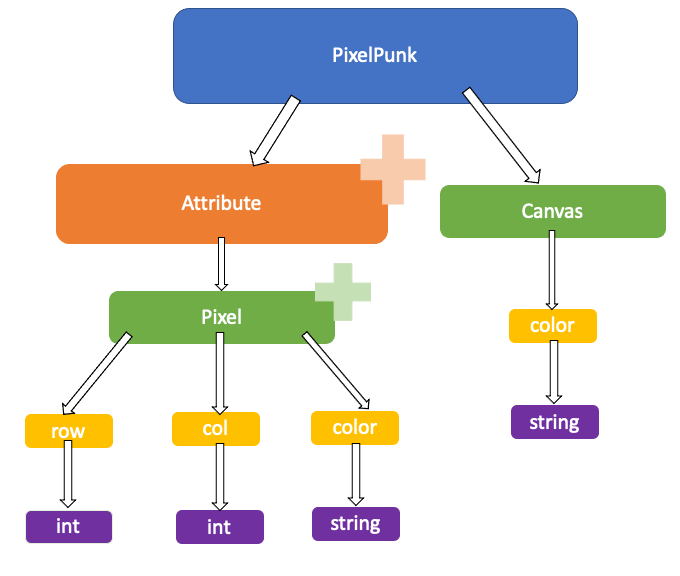
\includegraphics[width=0.75\textwidth]{images/hierachysketch.png}
    \end{center}
    
    \item To reiterate, pixels have a row, column, and color specifier, the canvas just takes a single color parameter, and everything else is just made of pixels. Below are the is the AST for the first example program.
    \begin{center}
    	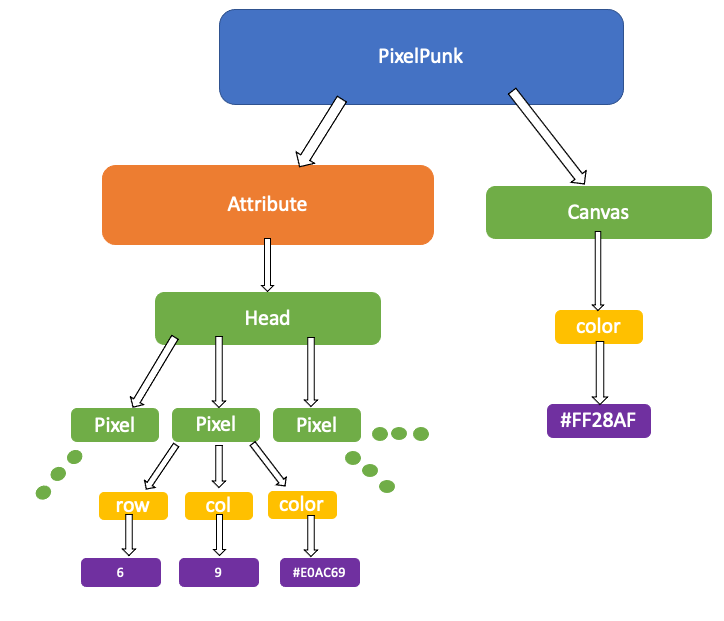
\includegraphics[width=0.75\textwidth]{images/ast1.png}
    \end{center}
    
    \item
        \begin{enumerate}
            \item Programs in this language do not read any input.
            \item The effect of evaluating a program is a 24x24 pixel grid in a svg file that is a pixel art profile picture.
            \item A post-order traversal of the AST would yield the described effect because we're essentially combining pixels into attributes and then combining attributes into PixelPunks.
            
            Ultimately, our evaluator will process the AST and output the PixelPunk grid as svg code into a PixelPunk.svg file, which can be opened easily in a browser such as Chrome for your viewing pleasure. 
        \end{enumerate}
    \end{enumerate}

\section{Remaining Work}

Our main goal for the end of this project is to create more pre-defined Attributes to make the PixelPunk language even more feature-rich and pleasant to use. We currently have optional Attributes like Hat and Sunglasses (in addition to Head, Eyes, Nose, and Mouth). However we plan to add even more accessories to make the diversity of feature options even greater. \\

As a stretch goal that extends beyond the scope of this class, we'd like to add the ability for users to easily mint their PixelPunks into NFTs using our programming language. This seems like the natural next step for our language.

% DO NOT DELETE ANYTHING BELOW THIS LINE
\end{document}
